\documentclass{standalone}
\usepackage{tikz}

\begin{document}

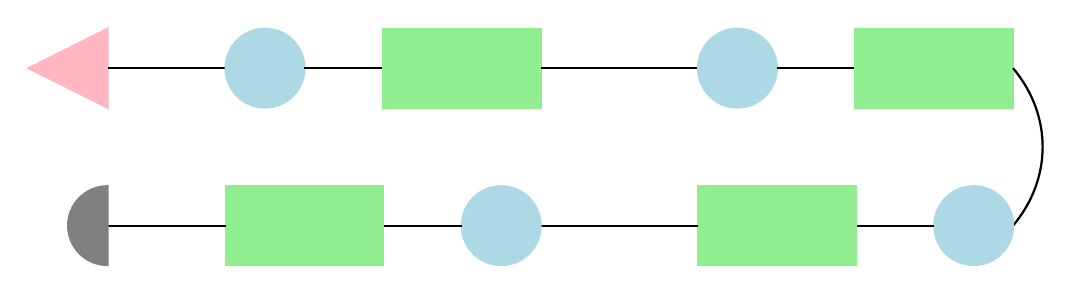
\begin{tikzpicture}

    % Define colors
    \definecolor{pastelblue}{RGB}{173,216,230}
    \definecolor{pastelyellow}{RGB}{255,255,204}
    \definecolor{pastelgreen}{RGB}{144,238,144}
    \definecolor{pastelred}{RGB}{255,182,193}

    \filldraw[pastelred, thick] (-3,0) -- (-2,0.5) -- (-2,-0.5) -- cycle;
    \draw[thick] (-2,0) to (0,0);

    \filldraw[pastelblue, thick] (0,0) circle(0.5);
    \draw[thick] (0.5,0) to (1.5,0);
    \filldraw[pastelgreen, thick] (1.5,0.5) rectangle (3.5,-0.5);

    \draw[thick] (3.5,0) to (5.5,0);

    \filldraw[pastelblue, thick] (6,0) circle(0.5);
    \draw[thick] (6.5,0) to (7.5,0);
    \filldraw[pastelgreen, thick] (7.5,0.5) rectangle (9.5,-0.5);

    %-------------
    \draw[thick] (9.5,0) to[out=-50,in=50] (9.5,-2);
    %-------------
    % Second row

    \filldraw[pastelblue, thick] (9,-2) circle(0.5);
    \draw[thick] (8.5,-2) to (7.5,-2);
    \filldraw[pastelgreen, thick] (5.5,-1.5) rectangle (7.5,-2.5);

    \draw[thick] (5.5,-2) to (3.5,-2);

    \filldraw[pastelblue, thick] (3,-2) circle(0.5);
    \draw[thick] (1.5,-2) to (2.5,-2);
    \filldraw[pastelgreen, thick] (-0.5,-1.5) rectangle (1.5,-2.5);


    \draw[thick] (-2,-2) to (-0.5,-2);
    \filldraw[gray, thick] (-2,-1.5) arc[start angle=90,end angle=270,radius=0.5] -- cycle;

\end{tikzpicture}

\end{document}
